\section{Introduction}
\subsection{Some Basic Mathematical Models}
We model many real-world situations using the language of differential equations. This may be the motion of a fluid, the current in an electric circuit, the position of a particle, the dissipation of heat, the price of a stock on the market, or just about anything one can imagine. \par
We use mathematical models to describe these real-world situations in ways that allow us to study them, or potentially solve them in some cases. The level of accuracy in these mathematical models can vary greatly, with more precise models being used when the situation calls for it. \par
For a basic example, consider the motion of a particle falling in a straight line. 
\begin{example}[Falling Object]
    One of the fundamental laws of physics, Newton's second law, states that the net force on an object is equal to the mass of the object times its acceleration:
    \[ F = ma \]
    An object falling on the surface of the earth will (in our model scenario) have two forces acting on it: gravity and air resistance. \par
    If we take the downwards direction (towards the surface of the earth) to be positive, gravity is a force given by
    \[ F_g = mg \]
    Where $g$ is a positive constant approximately equal to $9.81$ meters per second squared. Air resistance is a force given by
    \[ F_a = -kv^2 \]
    Where $k$ is a positive experimentally determined constant with units kilograms per meter, and $v$ is the velocity of the object. \par
    We can combine these equations to give us
    \[ ma = mg - kv^2 \]
    Taking notice that the acceleration of an object is the derivative of its velocity,
    \[ m\dv{v}{t} = mg - kv^2 \]
    Or, equivalently,
    \[ m \dv[2]{y}{t} = mg - k\pqty{\dv{x}{t}}^2 \]
    These two are examples of differential equations, which we will learn to solve. \par
    Although we cannot yet solve this equation, we are still able to analyze the equation in an attempt to shed some light on the behavior of the falling object.
\end{example}
\subsection{Direction Fields}
Direction fields are a tool that allow us to study the behavior of differential equations that can be written in the form
\[ \dv{y}{x} = f(x, y) \]
$f$ is sometimes called the \bf{rate function}. \par
We construct a direction field by creating a sketch of the $xy$ plane, and evaluating $f(x,y)$ at various points on the plane. At each point, we construct a small line segment that has a slope given by the value of $f(x,y)$ at that point. \par
To illustrate this, we will return to our previous example of an object falling under the influence of air resistance. 
\begin{example}[Direction Field of a Falling Object]
    We can begin to plug in some values to analyze our differential equation. For instance, if the object has a velocity of $v = 5$ meters per second, we find
    \[ m\dv{v}{t} = mg - k(5)^2 \]
    which tells us
    \[ \dv{v}{t} = g - \frac{25k}{m} \]
    If we plug in numerical values for $g$, $k$, and $m$, we get a number for $\dv{v}{t}$ with those specific values. If we repeat this process for many values of $v$, we can construct a direction field, as shown below. \par
    \begin{figure}[h!]
        \centering
        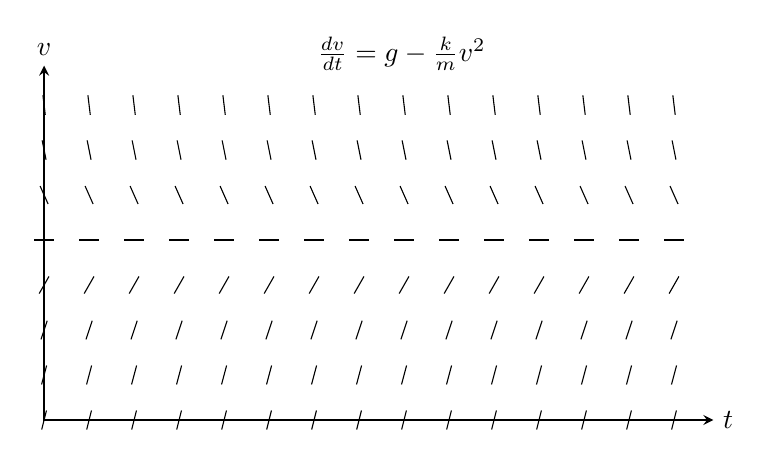
\begin{tikzpicture}
            
            \def\s{4}	 %size of axis
            \def\n{7}	 %number of points on axis
            \def\l{0.25} %length of direction lines
            
            %AXIS
            \draw[semithick,<->,>=stealth] (-\s,\s+0.5)--(-\s,0)--(\s+0.5,0);	  %quadrant 1
            % \draw[semithick,<->,>=stealth] (-\s,-\s-0.5)--(-\s,0);	
            %quadrant 4 (optional)
            \node[above] at (-\s,\s+0.5) {$v$};		\node[right] at (\s+0.5,0) {$t$};
            %
            %Write out your differential equation (optional):
            \node[right,align=left] at (-0.65,\s+0.65) {$\frac{dv}{dt} = g-\frac{k}{m}v^2$};
            
            \foreach \y in {0,...,\n}{	%all quadrants: {-\n,...,\n}; only first: {0,...,\n}
            \foreach \x in {-\n,...,\n}{	%NB: watch out for division by zero, e.g. dy/dx = -\y/\x
                \draw[rotate around={atan(% arctan converts from slope to degrees
                    4 - 0.25 *\y * \y	%  <-- RHS of differential equation goes here: dy\dx = ...
                ):(\x*\s/\n,\y*\s/\n)}] (\x*\s/\n-0.5*\l,\y*\s/\n)--++(\l,0);
            } %end of x loop
            } %end of y loop
        \end{tikzpicture}
    \end{figure}
    By following the ``flow'' of these lines, we can see how a curve of the velocity of an object versus time might look. Notice that there are many different possible curves that follow the direction field. Later, we will further explore how to narrow this family of possible curves to one specific one. \par
    One thing we can notice is that the velocity of the object approaches a fixed value as $t$ approaches $\infty$. This is called the ``terminal velocity'' of the object and is a natural consequence of our differential equation. If we plug in $v = \sqrt{\frac{mg}{k}}$ into our differential equation, we find 
    \[ \dv{v}{t} = mg - k\pqty{\sqrt{\frac{mg}{k}}}^2 = 0 \]
    Which can be interpreted as saying that when the object's velocity reaches this critical value, it will completely stop accelerating and continue falling at a constant speed. \par
    Any $v$-value where a constant solution can exist is called a \bf{steady state} for the differential equation. \par
    Notice that there is no strict dependency on $t$ in our differential equation. This is represented in the direction field by the fact that all direction lines with the same $v$ value are identical, regardless of their $t$ value. These types of equations, called \bf{autonomous} differential equations, will be one of the major forms of differential equation we study.
\end{example}
\begin{example}[Population Growth]
    
Another example of a differential equation is the growth of a population. Ignoring factors like competition, predation, or scarcity of resources, the growth rate of a population will be roughly proportional to the current population. As an equation, we can describe this scenario with
\[ \dv{P}{t} = rP \]
where $r$ is a positive constant with units time$^{-1}$. $r$ is known as the \bf{growth rate}, and can be thought of as a factor describing how quickly or often members of the population reproduce. \par
Now, suppose that a predator of our population is suddenly introduced. For simplicity, imagine that the population of the predators is constant, and they eat at a constant rate. This introduces a new factor to the differential equation, representing the rate at which the population decreases due to this predator. This gives us an updated differential equation of
\[ \dv{P}{t} = rP - k\]
where $k$ is a positive constant with units population per time. A higher $k$ value corresponds to a larger amount of predation. \par
We can gleam some understanding of this situation by analyzing the sign of $\dv{P}{t}$. If $rP > k$, then the population is growing. In this scenario, $rP$ will only continue to increase as the population grows, quickly leading to an out-of-control exponential growth. If $rP < k$, then the population is declining, and will only continue to decline faster until it reaches zero (technically, the equation dictates that $P$ continues to decline after it reaches zero, but we know that cannot happen because there can't be a negative population). If $rP = k$, then the population will be held at a constant value. \par
We can construct a direction field for our differential equation to ensure that it matches with the conclusions we have made from analyzing the equation. \par
\begin{figure}[h!]
    \centering
    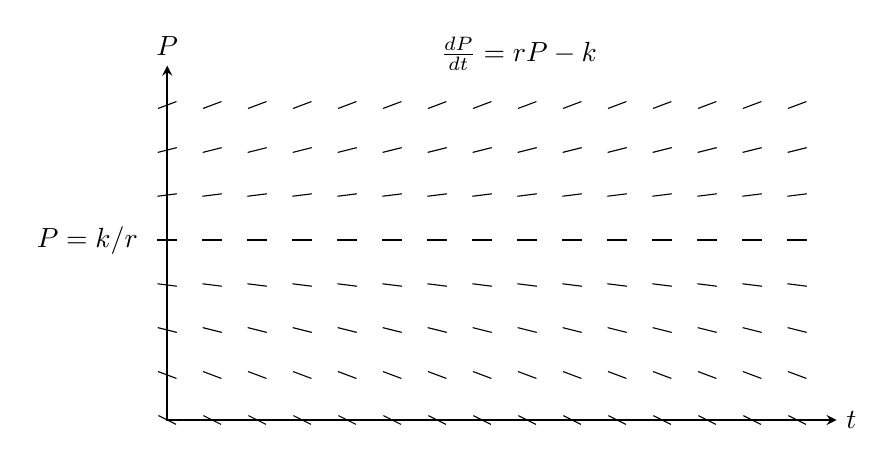
\begin{tikzpicture}
        
        \def\s{4}	 %size of axis
        \def\n{7}	 %number of points on axis
        \def\l{0.25} %length of direction lines
        
        %AXIS
        \draw[semithick,<->,>=stealth] (-\s,\s+0.5)--(-\s,0)--(\s+0.5,0);	  %quadrant 1
        % \draw[semithick,<->,>=stealth] (-\s,-\s-0.5)--(-\s,0);	
        %quadrant 4 (optional)
        \node[above] at (-\s,\s+0.5) {$P$};		\node[right] at (\s+0.5,0) {$t$};
        %
        %Write out your differential equation (optional):
        \node[right,align=left] at (-0.65,\s+0.65) {$\frac{dP}{dt} = rP - k$};
        \node[left, align=left] at (-\s - 0.25, \s * 0.57) {$P = k/r$};
        \foreach \y in {0,...,\n}{	%all quadrants: {-\n,...,\n}; only first: {0,...,\n}
        \foreach \x in {-\n,...,\n}{	%NB: watch out for division by zero, e.g. dy/dx = -\y/\x
            \draw[rotate around={atan(% arctan converts from slope to degrees
                0.125*\y - 0.5	%  <-- RHS of differential equation goes here: dy\dx = ...
            ):(\x*\s/\n,\y*\s/\n)}] (\x*\s/\n-0.5*\l,\y*\s/\n)--++(\l,0);
        } %end of x loop
        } %end of y loop
    \end{tikzpicture}
\end{figure}
This supports what we have previously found. There is a steady state solution at $P = k/r$. Anything below that decreases to zero and anything above that increases to infinity. 
\end{example}
You may have noticed that although the previous two examples both had a steady state solution where the dependent variable remains constant, the behavior around the steady state solution varied greatly. In the first example, solutions tended to approach the steady state, curving towards it. In the second example, however, the curves tended to leave the steady state, curving away from it. \par
In the first case, we call the steady state a \bf{stable equilibrium} due to the tendency of nearby solutions to gravitate towards it it. We call the second case an \bf{unstable equilibrium} due to the tendency of nearby solutions to be repelled away. \par
There is also a third type of equilibrium, where it is stable in one direction and unstable in the other. This is known as a \bf{semi-stable equilibrium}, and an example is pictured below. \newpage
\begin{figure}[h!]
    \centering
    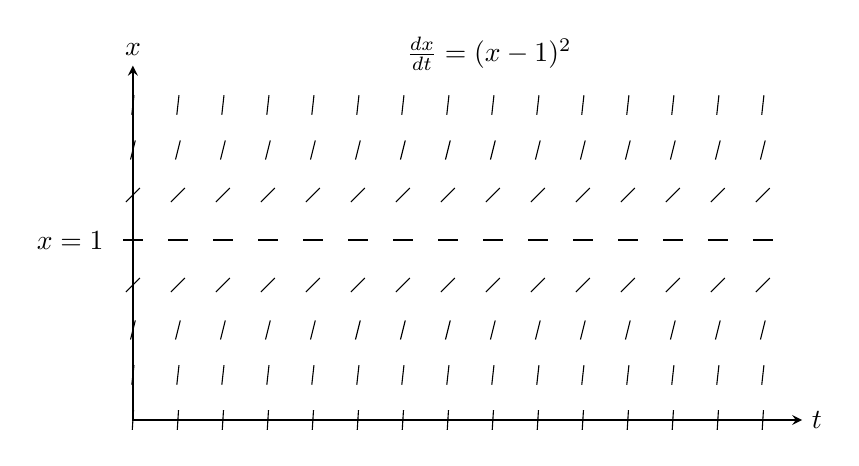
\begin{tikzpicture}
        
        \def\s{4}	 %size of axis
        \def\n{7}	 %number of points on axis
        \def\l{0.25} %length of direction lines
        
        %AXIS
        \draw[semithick,<->,>=stealth] (-\s,\s+0.5)--(-\s,0)--(\s+0.5,0);	  %quadrant 1
        % \draw[semithick,<->,>=stealth] (-\s,-\s-0.5)--(-\s,0);	
        %quadrant 4 (optional)
        \node[above] at (-\s,\s+0.5) {$x$};		\node[right] at (\s+0.5,0) {$t$};
        %
        %Write out your differential equation (optional):
        \node[right,align=left] at (-0.65,\s+0.65) {$\frac{dx}{dt} = (x-1)^2$};
        \node[left, align=left] at (-\s - 0.25, \s * 0.57) {$x = 1$};
        \foreach \y in {0,...,\n}{	%all quadrants: {-\n,...,\n}; only first: {0,...,\n}
        \foreach \x in {-\n,...,\n}{	%NB: watch out for division by zero, e.g. dy/dx = -\y/\x
            \draw[rotate around={atan(% arctan converts from slope to degrees
                \y * \y - 8 * \y + 16	%  <-- RHS of differential equation goes here: dy\dx = ...
            ):(\x*\s/\n,\y*\s/\n)}] (\x*\s/\n-0.5*\l,\y*\s/\n)--++(\l,0);
        } %end of x loop
        } %end of y loop
    \end{tikzpicture}
\end{figure}
Notice that $x$ tends towards the steady state from below, but away from the steady state from above.
\subsection{Solutions to Separable Differential Equations} \label{separablesection}
Some of the simplest differential equations to solve are known as separable first order differential equations. Separable first order equations can be written in the form
\[ \dv{x}{t} = f(x)g(t) \]
That is, we have the first derivative equal to the product of a a pure function of $x$ and a pure function of $t$. If $f(x) \neq 0$, we can rearrange to obtain
\[ \frac{1}{f(x)}\dv{x}{t} = g(t) \]
and then integrate both sides with respect to $t$ to find
\[ \int \frac{1}{f(x)}\dv{x}{t}\dd t = \int g(t) \dd t \]
or, equivalently,
\[ \int \frac{1}{f(x)}\dd x = \int g(t)\dd t \]
This gives you an implicit definition of $x(t)$, which can be found explicitly by evaluating the antiderivatives and performing algebra, as necessary. 
\begin{example}[Population Growth]
    Let's revisit our previous example of population growth. Recall that the differential equation governing the population $P$ of an animal species with growth rate $r$ and predation rate $k$ is 
    \[ \dv{P}{t} = rP - k \]
    With some algebra, we find 
    \[ \frac{1}{rP - k}\dv{P}{t} = 1 \]
    Then, we can integrate both sides and perform some algebra.
    \begin{align*}
        \int \frac{1}{rP - k}\dv{P}{t}\dd t &= \int \dd t \\
        \frac{1}{r}\ln \abs{rP - k} &= t + C \\
        rP - k &= \pm e^{rt + C}
    \end{align*}
    Because $C$ is just an arbitrary positive constant, we can redefine $rC = C_2$, which is just another constant. Although it is technically not mathematically sound, we will skip the process of renaming the arbitrary constant and just absorb the factor of $r$ into $C$. In the future, we will perform operations like this on arbitrary constants without commenting on it.
    \begin{align*}
        P &=  \pm\frac{1}{r}e^{rt + C} + \frac{k}{r} \\
        &= \pm \frac{1}{r}e^C e^{rt} + \frac{k}{r} \\
        &= Ce^{rt} + \frac{k}{r}
    \end{align*}
    This arbitrary constant $C$ is the reason why solutions to differential equations are a family of curves rather than a single function. What we have now is known as the \bf{general solution}, and describes all possible solutions to the equation. To narrow down to a single function, called the \bf{particular solution}, we must have an \bf{initial condition}. For instance, if we have $P(0) = P_0$, we can write
    \[ P(0) = P_0 = C + \frac{k}{r} \]
    which tells us that
    \[ C = P_0 - \frac{k}{r} \]
    and
    \[ P(t) = \pqty{P_0-\frac{k}{r}}e^{rt} + \frac{k}{r} \]
    We can verify that this equation satisfies $\dd P/\dd t = rP - k$ by computing its first derivative:
    \[ \dv{P}{t} = r\pqty{P_0 - \frac{k}{r}}e^{rt} = rP(t) - k \]
\end{example}
Another way to write separable differential equations is in the \bf{differential form}. If we take our original definition of a first order separable equation
\[ \dv{x}{t} = f(x)g(t)\]
we can rewrite it in the form
\[ M(t) + N(x)\dv{x}{t} = 0\]
Where $M(t) = -g(t)$ and $N(x) = 1/f(x)$. \par
We don't have the tools to formally mathematically justify this next step, because working with differentials is a bit advanced. However, it is allowed. \par 
We can multiply both sides of the equation by $\dd t$ to get
\[ M(t)\dd t + N(x)\dd x = 0 \] 
This new form is useful for some applications and numerical methods.
\subsection{Classification of Differential Equations}
\subsubsection{Ordinary and Partial Differential Equations}
There are two primary classes of differential equations--\bf{ordinary differential equations} and \bf{partial differential equations}. Ordinary differential equations (ODEs) are the ones we are concerned with in these notes. ODEs describe scenarios that are modeled by functions of one variable. For example, the charge on a capacitor in an electric circuit consisting of one inductor, capacitor, battery, and resistor can be modeled by a function of time $Q(t)$. The differential equation for this is
\[ L\dv[2]{Q(t)}{t} + R\dv{Q(t)}{t} + \frac{1}{C}Q(t) = \mathcal{E}(t) \]
where $L$, $R$, and $C$ are positive constants and $\mathcal{E}(t)$ describes the voltage of the battery as a function of time. \par
Partial differential equations, on the other hand, model scenarios with a function of two or more variables. For example, the wave equation $E(x,t)$ of an electric wave is described by
\[ \pdv[2]{E(x,t)}{x} = \frac{1}{c^2}\pdv[2]{E(x,t)}{t}\]
where $c$ is a positive constant equal to the speed of light. \par
Another subject of study that involves differential equations is the idea of systems of differential equations. These arise when there are two or more unknown variables modeled by a differential equation. We will explore these further later, but for a system of two differential equations, we may find something of the form
\begin{align*}
    \dv{x}{t} &= f(x,y,t) \\
    \dv{y}{t} &= g(x,y,t)
\end{align*}
\subsubsection{Order, Linear, and Nonlinear Equations}
One useful metric for analyzing differential equations is the order of an equation. The order of a differential equation is simply the highest derivative that appears in the equation. The equation
\[ F\pqty{t, x(t), x'(t), \cdots, x^{(n)}(t)} = 0\]
is the general expression of an $n^{\text{th}}$ order differential equation. We will usually assume that the previous expression can be rewritten to isolate the highest order derivative; that is, it can be written as
\[ x^{(n)}(t) = f\pqty{t, x(t), x'(t), \cdots, x^{(n-1)}(t)}\]
We make this assumption to avoid ambiguity. For instance, the differential equation
\[ a_3(y,t)\pqty{y'}^2 + a_2(y,t)y' + a_1(y,t) = 0\]
leads to two distinct equations:
\[ y' = \frac{-a_2(y,t) + \sqrt{\pqty{a_2(y,t)}^2-4\pqty{a_3(y,t)}\pqty{a_1(y,t)}}}{2a_3(y,t)}\quad\text{and}\quad y'=\frac{-a_2(y,t) - \sqrt{\pqty{a_2(y,t)}^2-4\pqty{a_3(y,t)}\pqty{a_1(y,t)}}}{2a_3(y,t)}\]
Another classification of differential equations that will prove useful is the notion of linear and nonlinear equations. An $n^{\text{th}}$ order differential equation is said to be \bf{linear} if it can be written in the form
\[ a_n(t)y^{(n)} + \cdots + a_2(t)y'' + a_1(t)y' = g(t) \]
That is, all coefficients of the $y$ terms depend only on $t$. Otherwise, it is called \bf{nonlinear}. All of the differential equations we have seen thus far are linear. An example of a nonlinear equation is
\[ y y' + 2y = e^t\]
This is nonlinear because the coefficient of the $y'$ term does not depend solely on $t$. \par
The methods and theory behind solving linear equations is very well-developed, while the methods for solving nonlinear equations is comparatively primative. \par
An example of a nonlinear system is the motion of a ball oscillating on a pendulum. With some trigonometry and analysis of the forces on the pendulum, we arrive at the differential equation
\[ \dv[2]{\theta}{t} + \frac{g}{L}\sin\theta = 0\]
where $L$ is the length of the pendulum and $\theta$ is the angle the pendulum makes with the vertical axis. This equation is nonlinear due to the $\sin\theta$ term, and does not have a nice solution due to its nonlinearity. Instead, physicists have used the approximation $\sin\theta \approx \theta$ for small values of $\theta$ to approximate the behavior of the system with the linear differential equation
\[ \dv[2]{\theta}{t} + \frac{g}{L}\theta = 0 \]
The process of approximating the behavior of a nonlinear system with a linear one is known as \bf{linearization}.
\subsection{Solutions of Differential Equations}
We already have a basic understanding of what it means for a function to solve a differential equation. It will be useful, however, to put it into more precise language. 
\begin{definition}
    Suppose there exists an $n^{\text{th}}$ order differential equation given by
    \[ x^{(n)}(t) = f\pqty{t, x(t), x'(t), \cdots, x^{(n-1)}(t)} \]
    where each $x^{(i)}$ is defined on some common domain $D$. Then, a
    \bf{solution} to the equation on an interval $[a, b]\subset D$ is any function $\varphi(t)$ such that
    \[ \varphi^{(n)}(t) = \pqty{t, \varphi(t), \varphi'(t), \cdots, \varphi^{(n-1)}(t)} \]
    is satisfied for all $t\in [a,b]$.
\end{definition}
One important thing to note about this definition is that solutions are only defined on \bf{connected} intervals. So, for example, if a discontinuity in the equation exists at $t=0$, there are no solutions on the domain $(-\infty, 0)\cup (0, \infty)$. Instead, solutions can only exist on each half of the interval--$(-\infty, 0)$ or $(0, \infty)$, or subsets of these intervals.
